\section{The Cactaceae}

There are approximately 130 genera and 2000 species in the Cactaceae family (order Caryophyllales); all of which are indigenous to the Americas \citep{Anderson2001, Wallace2002, Zimmermann2009, Novoa2015IntroducedReview, christenhusz2016number}. The one exception is the epiphyte \textit{Rhipsalis baccifera} Stern (`mistletoe cactus'), which is possibly native to southern Africa and Madagascar \citep{Wallace2002, Zimmermann2009}. The centre of cactus diversity in the native range is in Mexico, where the three most speciose genera are \textit{Opuntia}, \textit{Echinopsis}, and \textit{Mammillaria} \citep{Novoa2015IntroducedReview}. The Cactaceae family evolved about 65 mya in South America \citep{Anderson2001}, and radiated about 30 to 35 mya in response to the aridification of the Americas and increased atmospheric CO\textsubscript{2} \citep{Arakaki2011, Majure2012}. The Cactaceae comprise four subfamilies; namely the Pereskioideae, Cactoideae, Maihuenioideae, and Opuntioideae \citep{Labra2003}. Their distribution spans from southern Patagonia in Argentina to British Columbia in Canada \citep{Anderson2001, Edwards2005}. Most cactaceous plants are succulents and are adapted to extreme xeric environments, although some epiphytes have even been found to thrive in rain forests \citep{Anderson2001}. Most species possess leafless photosynthetic stems and protective spines, which are modified leaves arising from areoles \citep{eggli1993glossary}. The spines of cactaceous plants are adapted for a number of functions across different species, such as protection from herbivores, camouflage, thermoregulation, water conservation, and dispersal \citep{Anderson2001}.
The Cactaceae display a diverse range of growth forms and sizes, from the smallest species (\textit{Blossfeldia liliputana} Werdermann) measuring 9 mm in diameter to one of the largest that stands nearly 20 m tall (\textit{Pachycereus pringlei} Britton \& Rose, the `Giant Mexican cardon') \citep{Anderson2001}. Some botanists have classified 13 different growth forms within this family, ranging from globular and columnar, to leaf-like and clustering \citep{Anderson2001}. Cactaceous plants typically display a diploid chromosome system of 2n = 22, but numerous species in the Opuntioideae family are known to display polyploidy \citep{Anderson2001}. Additionally, asexual reproduction is common in many Cactaceae, where stem joints can break off the main plant, grow adventitious roots, and give rise to new plants \citep{Anderson2001}. \\
Although the Cactaceae are endemic to the New World, they have become naturalised widely outside their native distribution, and, in many cases, have become serious invaders \citep{Novoa2015IntroducedReview}. Of the 1922 cactus species reviewed by \citet{Novoa2015IntroducedReview}, 57 (3\%) were invasive in other parts of the world (Fig. \ref{fig:novoaMap}). The review reported that \textit{O. ficus-indica} was the most widespread invader; having been recorded in 22 countries outside its native range. The countries most heavily invaded by cactaceous weeds are Australia, South Africa, and Spain; with 39, 35, and 24 recorded species, respectively.
\vspace{0.4cm}

\begin{figure}[H]
	\centering
	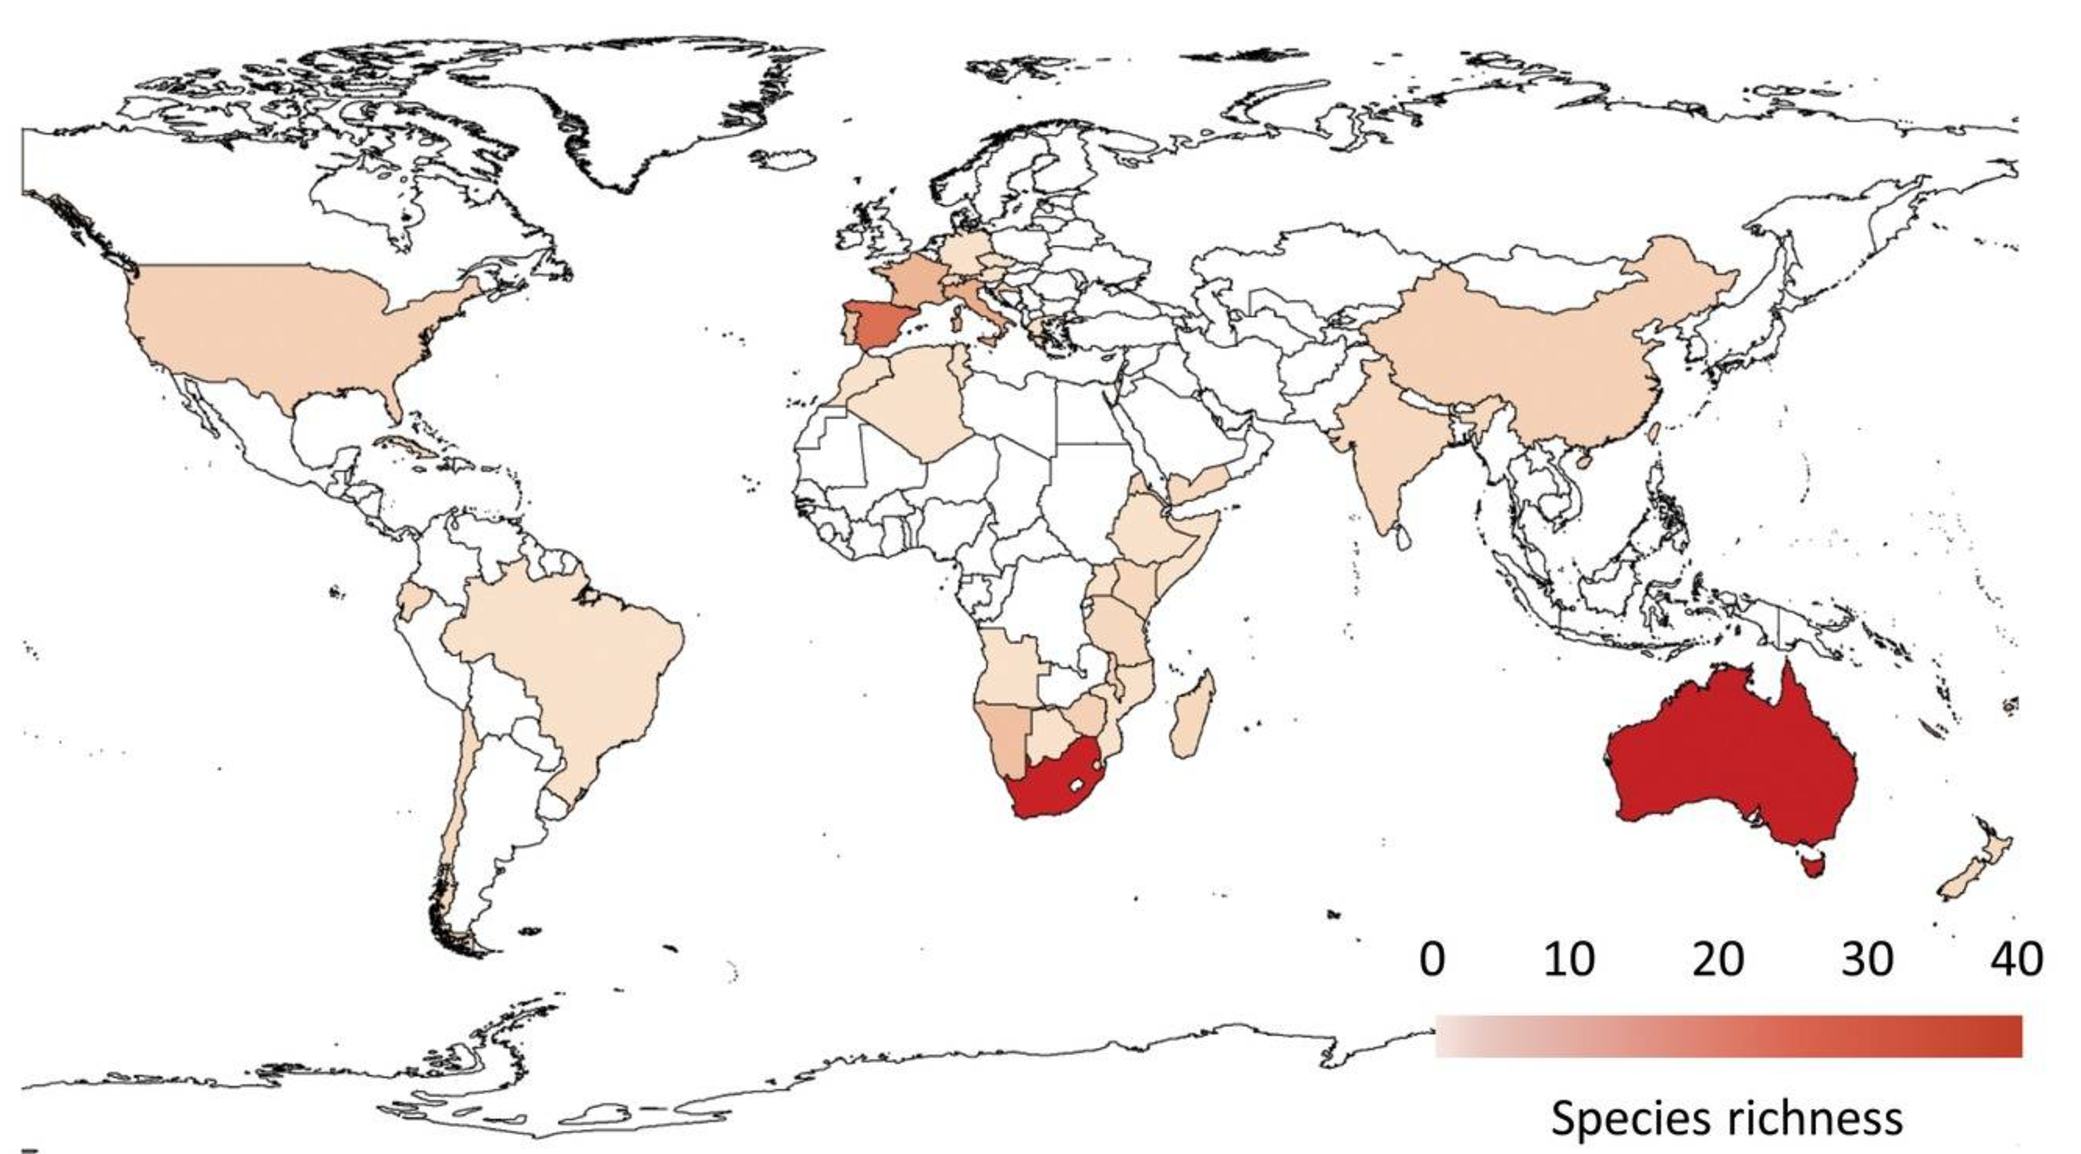
\includegraphics[scale = 0.45]{Images/novoa_map.pdf}
	\caption{The invasive range of 57 cactus species, as reviewed by \citet{Novoa2015IntroducedReview}.}
	\label{fig:novoaMap}
\end{figure}

\subsection{Biological control of invasive Cactaceae}

The two predominant countries implementing cactus biocontrol are South Africa and Australia \citep{Moran1991a, paterson2019prospects}.
Numerous cactus species were introduced to these countries as ornamental and hedge plants, as a source of fruit and fodder, and for the establishment of a red dye industry during their early colonial periods \citep{Zimmermann2009, Paterson2011BiologicalAfrica, kaplan2017proposed, managingOpuntioid2017} (Tables \ref{tab:invasiveCactiSA} and \ref{tab:invasiveCactiAus}). There are four main groups of invasive cacti: namely the `platyopuntia' (e.g. \textit{Opuntia ficus-indica, O. stricta}, and \textit{O. monacantha}), `cylindropuntia' (e.g. \textit{Cylindropuntia imbricata}), `organ-pipe' (e.g. \textit{Harrisia martinii} and \textit{Cereus jamacaru}), and `leafy' (e.g. \textit{Pereskia aculeata}) \citep{Klein2002WeedsBiocontrol}. The main adaptations enabling the invasibility of these plants are their:
\vspace{0.4cm}
\begin{enumerate}
    \item Tolerance to xeric conditions and their water-efficient CAM (Crassulacean Acid Metabolism) photosynthetic strategy.
    \item Ability to outcompete native vegetation under disturbed conditions.
    \item Ability to reproduce both sexually and asexually. \\ \citep{Zimmermann2009}.
\end{enumerate}
\vspace{0.4cm}

\noindent Approximately 400 cactus taxa have been introduced to South Africa \citep{kaplan2017proposed}, of which 35 species are invasive \citep{Novoa2015IntroducedReview}. Twenty three of these have been subject to biological control using 19 insect species \citep{Zimmermann2009, Klein2011,Paterson2011BiologicalAfrica}. Of these, four are under complete control (\textit{Cereus jamacaru} D. C., \textit{Cylindropuntia fulgida} Engelmann, \textit{C. leptocaulis} Knuth, and \textit{Harrisia martinii} Labour) and eight are under substantial control (\textit{Cylindropuntia imbricata} Haworth, \textit{Harrisia balansae} (K.Schum.)  N. P. Taylor \& Zappi, \textit{Opuntia aurantiaca} Lindley, \textit{O. engelmannii} Salm-Dyck ex. Engelm., \textit{O. ficus-indica} (L.) Mill., \textit{O. monacantha} Haworth. \textit{O. salmiana} J. Parm. ex Pfeiff, and \textit{O. stricta}  Haworth) \citep{Klein2011}. \\
From 1920 to 1935, the Australian government funded the importation of 52 different potential cactus biocontrol agents for host specificity testing; of which 12 were released \citep{raghu2007understanding}. These included multiple \textit{Dactylopius} species, two \textit{Chelinidea} spp. (Hemiptera: Coreidae), an \textit{Olycella} sp. (Lepidoptera: Pyralidae), and \textit{Tetranychus opuntiae} (Acari: Tetranychidae) \citep{raghu2007understanding}. Additionally, \textit{Cactoblastis cactorum} (Lepidoptera: Pyralidae) was released in 1925 and established successfully \citep{mann1970cacti}; destroying hundreds of hectares of \textit{Opuntia}-infested areas within two years \citep{raghu2007understanding}.
Australia currently has 39 recorded invasive cactus taxa belonging to four genera; and is the most heavily invaded of all the countries surveyed by \citet{Novoa2015IntroducedReview}. Twenty-seven species are listed in the Weeds of National Significance (WoNS) database (Table \ref{tab:invasiveCactiAus}) \citep{managingOpuntioid2017}. Of the naturalised species, \textit{Corynopuntia} sp., \textit{O. dejecta}, and \textit{O. ficus-indica} are not considered invasive \citep{managingOpuntioid2017}. The two most prominent biological control agents in use are \textit{C. cactorum} and four \textit{Dactylopius} species; namely \textit{D. austrinus}, \textit{D. ceylonicus}, \textit{D. opuntiae}, and four \textit{D. tomentosus} lineages \citep{managingOpuntioid2017}. \\
The absence of indigenous Cactaceae and its relatives outside the New World allows for the use of less host-specific (oligophagous) agents in invaded areas, as there is a lower risk of non-target attack \citep{Zimmermann2002}. This also means that multiple target weeds can be attacked by oligophagous agents \citep{paterson2019prospects}. \\

\begin{table}[H]
\caption{National Environmental Management: Biodiversity Act (NEM:BA) Category 1 and 2 invasive cactus species in South Africa. Category 1a and 1b weeds require compulsory control, and need to be removed and destroyed. Category 2 weeds are regulated by area, and require demarcation permits (none are, however, allowed in riparian zones) \citep{nemba}.} \label{tab:invasiveCactiSA} 
\renewcommand{\arraystretch}{0.5}
\resizebox{\columnwidth}{!}{%
\begin{tabular}{@{}lll@{}}
\toprule
\textbf{Species} & \textbf{Common name} & \textbf{Category} \\ \midrule
\textit{Austrocylindropuntia cylindrica} (Juss. ex Lam.) Backeberg. & Cane cactus & 1a \\
\textit{Austrocylindropuntia subulata}
(Muehlenpf.) \\ Backeb. subsp. exaltata 
(A. Berger) D. R. Hunt & Long spine cactus & 1b \\
\textit{Cereus hexagonus} (L.) Mill. & Queen of the night & 1b \\
\textit{Cereus hildmannianus} K. Schum. & Queen of the night & 1b \\
\textit{Cerues jamacaru} D. C. & Queen of the night & 1b \\
\begin{tabular}[c]{@{}l@{}}\textit{Cylindropuntia fulgida} (Engelm.)\\ F. M. Knuth var. \textit{fulgida} \end{tabular} & Chain-fruit cholla & 1b \\
\begin{tabular}[c]{@{}l@{}}\textit{Cylindropuntia fulgida} (Engelm.)\\ F. M. Knuth var. \textit{mamillata} (Schott ex\\ Engelm.)\end{tabular} & Boxing glove cactus & 1b \\
\begin{tabular}[c]{@{}l@{}}\textit{Cylindropuntia imbricata} (Haw.)\\ F. M. Knuth\end{tabular} & Imbricate cactus & 1b \\
\textit{Cylindropuntia leptocaulis} (D. C.) F. M. Knuth & Pencil cactus & 1b \\
\textit{Cylindropuntia pallida} (Rose) F. M. Knuth & Pink-flowered sheathed cholla & 1a \\
\textit{Cylindropuntia spinosior} (Englem.) F. M. Knuth & Cane cholla & 1a \\ 
\textit{Harrisia balansae} (K. Schum.) N. P. Taylor \& Zappi & Strangler prickly apple & 1a \\ 
\textit{Harrisia martinii} (Labour.) Britton & Moon cactus & 1b \\
\textit{Harrisia pomanensis} (F. A. C. Weber) Britton \& Rose & Midnight lady & 1a \\
\textit{Harrisia tortuosa} (J. Forbes ex Otto \& A. Dietr.) \\ Britton \& Rose & Spiny snake cactus & 1b \\
\textit{Hylocereus undatus} (Haw.) Britton \& Rose & Night-blooming cereus & 2 \\
\textit{Myrtillocactus geometrizans} (Mart.) Console & Bilberry cactus & 1a \\
\textit{Opuntia aurantiaca} Lindl. & Jointed cactus & 1b \\
\textit{Opuntia elata} Link \& Otto ex Salm-Dyck & Orange tuna & 1b \\
\textit{Opuntia engelmannii} Salm-Dyck ex Engelm. & Small round-leaved prickly pear & 1b \\
\textit{Opuntia ficus-indica} (L.) Mill. & Sweet prickly pear & 1b \\
\textit{Opuntia humifusa} (Raf.) Raf & Creeping prickly pear & 1b \\
\textit{Opuntia leucotricha} D. C. & Aaron's-beard prickly pear & 1b \\
\textit{Opuntia microdasys} (Lehm.) Pfeiff & Yellow bunny-ears & 1b \\
\textit{Opuntia monacantha} Haw & Drooping prickly pear & 1b \\
\textit{Opuntia pubescens} J. C. Wendl. ex Pfeiff. & Velvet bur cactus & 1a \\
\textit{Opuntia robusta} H. L. Wendl. ex Pfeiff & Blue-leaf cactus & 1a \\
\textit{Opuntia salmiana} J. Parm. ex Pfeiff & Bur cactus & 1a \\
\textit{Opuntia spinulifera} Salm-Dyck & Saucepan cactus & 1b \\
\textit{Opuntia stricta} (Haw.) Haw. var. \textit{stricta} \\
and var. \textit{dillenii} (Ker Gawl.) L. D. Benson  & Pest pear of Australia & 1b \\
\textit{Opuntia tomentosa} Salm-Dyck & Velvet opuntia & 1b \\
\textit{Peniocereus serpentinus} (Lag. \& Rodr.) N. P. Taylor & Serpent cactus & 1b \\
\textit{Pereskia aculeata} Mill. & Barbados gooseberry & 1b \\
\textit{Tephrocactus articulatus} (Pfeiff.) Backeb. & Pine cone cactus & 1a \\
\bottomrule
\end{tabular}
}
\end{table}

\clearpage

\begin{table}[H]
\caption{List of the Cactaceae in the Australian Weeds of National Significance (WoNS) database \citep{managingOpuntioid2017}.} \label{tab:invasiveCactiAus} 
\renewcommand{\arraystretch}{0.5}
\centering
\begin{tabular}{@{}ll@{}}
\toprule
\textbf{Species} & \textbf{Common name} \\ \midrule
\textit{Austrocylindropuntia cylindrica} & Cane cactus \\
\textit{Austrocylindropuntia subulata} & Eve’s needle cactus \\
\textit{Cylindropuntia fulgida var. mamillata} & Coral cactus \\
\textit{Cylindropuntia imbricata} & Devil’s rope \\
\textit{Cylindropuntia kleiniae} & Klein's cholla \\
\textit{Cylindropuntia leptocaulis} & Pencil cactus \\
\textit{Cylindropuntia pallida} & White-spined Hudson pear \\
\textit{Cylindropuntia prolifera} & Jumping cholla \\
\textit{Cylindropuntia spinosior} & Snake cactus \\
\textit{Cylindropuntia tunicata} & Brown-spined Hudson pear \\
\textit{Opuntia aurantiaca} & Tiger pear \\
\textit{Opuntia elata} & Riverina pear \\
\textit{Opuntia elatior} & Red-flower prickly pear \\
\textit{Opuntia engelmannii} & Engelmann's prickly pear \\
\textit{Opuntia humifusa} &  \\
\textit{Opuntia leucotricha} &  \\
\textit{Opuntia microdasys} & Bunny ears \\
\textit{Opuntia sp. aff. microdasys} &  \\
\textit{Opuntia monacantha} & Drooping tree pear \\
\textit{Opuntia aff. polyacantha} &  \\
\textit{Opuntia puberula} &  \\
\textit{Opuntia robusta} &  \\
\textit{Opuntia schickendantzii} &  \\
\textit{Opuntia streptacantha} & Westwood pear \\
\textit{Opuntia stricta} var. \textit{stricta} and var. \textit{dillenii} &  \\
\textit{Opuntia sulphurea} &  \\
\textit{Opuntia tomentosa} & Velvet tree pear \\ \bottomrule
\end{tabular}
\end{table}

\subsubsection{\textit{Opuntia} Mill}

The \textit{Opuntia} genus is the most widespread of all the cacti, comprising approximately 180 species and numerous hybrids \citep{Anderson2001, Griffith2003}. \textit{Opuntia ficus-indica} L. (`sweet prickly pear') was likely one of the first cactus species introduced to South Africa in the early 1700s, and became widespread throughout the Karoo and Eastern Cape by the 1800s \citep{Annecke1978, Dean2000}. 
Numerous spineless varieties were bred in the early 1900s by the horticulturist Luther Burbank, and exported around the world as a source of food and fodder for livestock, and for its fruit \citep{anderson2015vast}. The first record of an \textit{Opuntia} species in Australia was in 1788, when the British brought both \textit{O. monacantha} and \textit{Dactylopius} species into the country to establish a red dye industry \citep{mann1970cacti}.
Many more \textit{Opuntia} species were introduced over the next few decades, and proceeded to cause major environmental damage and economic losses to the agricultural sectors in South Africa and Australia due to the growth of dense, impenetrable thickets on farmlands \citep{Dean2000}. \citet{novoa2019spinelessness} showed that spineless varieties grown from seeds (i.e. sexual reproduction) reverted back to their spiny form, which explains their high incidence in invaded regions. 
Mechanical and chemical control methods were initially implemented to control the weed, particularly the use of arsenical herbicides such as injectable monosodium methanearsonate (MSMA) \citep{Annecke1978,Zimmermann1991BiologicalAfrica}. \\ \textit{Opuntia stricta} Haworth (var. \textit{stricta}) (`Australian pest pear') was first recorded in Australia in 1839, and spread at a rate of 320 000 ha per year (at densities of about 250 000 kg per ha!) by the 1920s \citep{raghu2007understanding}. \textit{Dactylopius ceylonicus} was initially released to combat the weed in 1903, but did not establish because this insect is host-specific to \textit{O. monacantha}. The later release of the \textit{D. opuntiae} `stricta' lineage in 1921 caused substantial damage \citep{Winston2014BiologicalWeeds.}.
Following the success of the biological control of \textit{Opuntia stricta} Haworth (both subspecies, nameley var. \textit{stricta} and var. \textit{dillenii}) and \textit{O. ficus-indica} L. in Australia, four insects were successfully released in South Africa as an additional means to control the weed \citep{Annecke1978,Zimmermann1991BiologicalAfrica}. These were the cladode boring moth \textit{C. cactorum} Berg (Lepidoptera: Pyralidae) released in 1933, the cladode sucking cochineal bug \textit{D. opuntiae} (`ficus' lineage) Cockerell (Hemiptera: Dactylopiidae) released in 1938, and the stem boring beetles \textit{Lagocheirus funestus} Thompson (Coleoptera: Cerambycidae) released in 1943 and \textit{Metamasius spinolae} Gyllenhal (Coleoptera: Curculionidae) released in 1948 \citep{Klein2011}. Of these, \textit{C. cactorum}, and particularly \textit{D. opuntiae}, have been the most effective agents - to the point that the agents themselves were seen as a threat to commercial \textit{O. ficus-indica} plantations \citep{Zimmermann1991BiologicalAfrica}. This is currently the case in Brazil, Israel, and the Mediterranean area, where \textit{D. opuntiae} is threatening and/or causing substantial losses to the cactus fodder and fruit industry \citep{spodek2014first, torres2018management, mazzeo2019dactylopius}. Conflicts of interest are common in the control of invasive Cactaceae \citep{novoa2016resolving}, and arise when an invasive species holds economic value in its introduced range. 
For example, \textit{Opuntia ficus-indica} L. (Mill.) provides a source of income for many rural communities in South Africa \citep{Brutsch1993ThePlants, Beinart2011}. The fruit is harvested and sold, and is also used to make beer, jam, and traditional medicines \citep{Brutsch1993ThePlants, shackleton2011invasive}. Rural communities in the Eastern Cape Province in particular rely heavily on the fruit for an income, and the local people are generally unaware of its invasive status  \citep{shackleton2007assessing}. Greater communication between these informal traders and the municipality is necessary, where legislation needs to be implemented that achieves a balance between limiting the negative effects of the invader on the environment, and promoting economic growth \citep{shackleton2011invasive}. \\ 
\textit{Opuntia stricta} became particularly problematic in the Kruger National Park in South Africa; where elephants, baboons, and rivers aid in its dispersal \citep{hoffmann1998long}. \textit{Cactoblastis cactorum} was released in the park in 1988 to control the weed  \citep{Hoffmann1998EvaluationAfrica}, followed by \textit{D. opuntiae} (`stricta' lineage) in 1997 \citep{Klein2011}. Both these insects established successfully, where a biomass reduction of over 90\%, and an almost complete end to fruit production, has been recorded \citep{Paterson2011BiologicalAfrica}. The weed is currently considered to be under substantial control \citep{Klein2011}. \\
\textit{Opuntia aurantiaca} Lindley, commonly referred to as `jointed cactus', is indigenous to Argentina and Uruguay, and is thought to be a hybrid of \textit{O. discolor} Britton \& Rose and \textit{O. salmiana} J. Parm ex. Pfeiff \citep{Moran1991BiologicalAfrica}. 
% The botanist John Lindley first described \textit{O. aurantiaca} in 1833, and incorrectly claimed that it was native to Chile based on a misinterpreation of a report by the avid British plant collector John Gillies \citep{moran1976}. The name `\textit{aurantiaca}' stems from the Latin word `auros', meaning `gold'. The name was based upon a manuscript by John Gillies in which he recorded a cactus plant with orange flowers occurring in Chile and Mendoza, Argentina. Subsequent confusion arose regarding the identity of the plant, as the flowers originally described by Lindley were bright yellow. The cacti with orange flowers turned out to be a misidentification, and were in fact \textit{O. longispina} var. \textit{corrugata} Backeberg \citep{moran1976}.  
It is now accepted that \textit{O. aurantiaca} is native to east Argentina and Uruguay \citep{DeLotto1974, gunn1979, zimmermann1981JointedCactus}.
The weed was introduced to South Africa as an ornamental plant in 1843 from collections in the United Kingdom \citep{zimmermann1981JointedCactus}, and later became problematic in grazing areas in the Karoo region and the Eastern Cape Province \citep{Moran1991BiologicalAfrica}.
The first biocontrol agent to be released on this weed in Australia and South Africa was \textit{D. austrinus} De Lotto (Hemiptera: Dactylopiidae) in 1933 and 1935, respectively \citep{Moran1991BiologicalAfrica, Winston2014BiologicalWeeds.}. Only \textit{D. austrinus} and \textit{C. cactorum} established successfully on the weed \citep{Klein2011}, while the other three attempted agents failed (\textit{Mimorista pulchellalis} Dyar (Lepidoptera: Crambidae), \textit{Nanaia} spp. (Lepidoptera: Pyralidae), and \textit{Zophodia tapiacola} Dyar (Lepidoptera: Pyralidae)). 

\subsubsection{\textit{Cylindropuntia} (Engelmann) (Knuth)}
The \textit{Cylindropuntia} genus (commonly known as `chollas') is a monophyletic clade that falls within the Opuntioideae subfamily \citep{Anderson2001}. It was originally classified as a subgenus of \textit{Opuntia} in 1856, but was later placed in its own genus in 1935 \citep{Anderson2001}. The genus comprises 33 species, and, as with many of the \textit{Opuntia} species, undergoes natural hybridisation \citep{Anderson2001}. 
\textit{Cylindropuntia imbricata} was first introduced to South Africa in the early 1900s \citep{Moran1991BiologicalAfrica}. 
The weed was successfully controlled in Australia by \textit{D. tomentosus} after its release in the country in 1925 \citep{Dodd1940}. South Africa followed suit and released the insect in 1970 \citep{Moran1991BiologicalAfrica}. The only other biocontrol agent associated with the weed, \textit{Metamasius spinolae}, did not establish successfully \citep{Klein2011}. \\
\textit{Cylindropuntia fulgida} (Engelm. Knuth) (‘chain fruit cholla’) is a tree-like cactus that comes in two varieties; namely var. \textit{fulgida} and var. \textit{mamillata} \citep{Anderson2001}. \textit{Cylindropuntia fulgida} var. \textit{fulgida} was introduced to South Africa in the 1940s as an ornamental plant \citep{DeBeer1986}, and has become particularly damaging to pastoral lands in the Northern Cape and Limpopo Provinces \citep{Moran1991BiologicalAfrica,Paterson2011BiologicalAfrica}. The cactus was initially misidentified as \textit{C. rosea}, and as a result, biocontrol efforts were largely unsuccessful due to a less effective \textit{D. tomentosus} lineage being released \citep{Paterson2011BiologicalAfrica}. Following the correct identification of the weed, various \textit{D. tomentosus} lineages were collected in Mexico; namely from the two \textit{C. fulgida} varieties and from \textit{C. cholla} (F.A.C. Weber) (Knuth) \citep{Paterson2011BiologicalAfrica}. It was found that the \textit{C. cholla} lineage was the most damaging, and hence became the agent of choice for this cactus variety \citep{Mathenge2009a}. Other category 1a and 1b species in this genus in South Africa are \textit{C. pallida}, \textit{C. spinosior}, and \textit{C. leptocaulis} (Table \ref{tab:invasiveCactiSA}). In addition to these, Australia has listed \textit{C. kleiniae}, \textit{C. prolifera}, and \textit{C. tunicata} in their WoNS database (Table \ref{tab:invasiveCactiAus}).